\section{Présentation}

Onyx est une plateforme à plugins généraliste, ce qui veut dire que la plateforme seule n'a aucun comportement mais qu'en ajoutant des plugins respectants les interfaces fournies on peut créer n'importe quelle application et comportement.
\\
\\
On peut utiliser la plateforme de deux manières:


\subsection{Lancement par défaut}

Lorsqu'on lance la plateforme sans aucun paramètres, elle va automatiquement charger les plugins référencés dans le fichier "default-plugins.xml"

\subsection{Lancement par commandes}

TO DO

\section{Structure}

\subsection{Diagramme de classe}
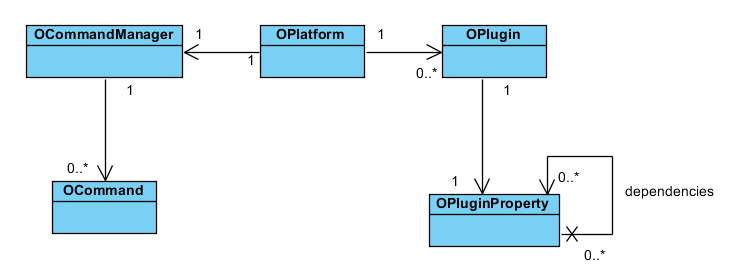
\includegraphics[width=15cm]{figures/class_diagram.png}
\newpage
\section{Installation}

Tout d’abord, dans un terminal, tapez:
\begin{verbatim}
git clone https://github.com/masters-info-nantes/onyx.git
\end{verbatim}

Lorsque tous les fichiers sont téléchargés,vérifiez que le proxy de maven est correct en faisant:
\begin{verbatim}
nano /.m2/settings.xml
\end{verbatim}

Le fichier devrait ressembler à ça:
\begin{verbatim}
<settings>
    <proxies>
        <proxy>
            <id>example-proxy</id>
            <active>true</active>
            <protocol>http</protocol>
            <host>proxy.ensinfo.sciences.univ-nantes.prive</host>
            <port>3128</port>
        </proxy>
    </proxies>
</settings>
\end{verbatim}

Placez-vous dans le dossier où vous avez cloné le projet. 
Tapez la commande:
\begin{verbatim}
mvn clean install
\end{verbatim}

Pour lancer l'execution par défaut, tapez:
\begin{verbatim}
mvn exec:java-X
\end{verbatim}

\newpage
\section{Plugins}

\subsection{Création d'un nouveau plugin}

Un plugin pour être intégré à la plateforme doit, comme vous vous en doutez, implémenter l'interface OPlugin comme ci-dessous:
\subsubsection{myMainClass.java}
\begin{verbatim}
package com.onyx.myPlugin;

import com.onyx.platform.OPlugin;
import com.onyx.platform.OPluginProperty;

public class myMainClass extends OPlugin{

    public myMainClass() {
        //Add some code here
    }

    @Override
    public void onCreate() {
        //Add some code here
    }

    @Override
    public void onStop() {
        //Add some code here
    }

}
\end{verbatim}

Pour que votre plugin soit correctement reconnu par la plateforme, vous devez lui fournir un fichier Omanifest sous cette forme:
Attention! Si vous définissez des dépendances pour le plugin, vous devez les inclure dans maven
\subsubsection{Omanifest}
\begin{verbatim}
<?xml version="1.0"?>
<manifest>
    <id>com.onyx.myPlugin</id>
    <version>0.1</version>
    <name>myPlugin</name>
    <descriptionplugin for onyx</description>
    <mainClass>com.onyx.myPlugin.myMainClass</mainClass>
    /* les dépendences ne sont pas obligatoires */
    <dependencies>
        <dependency>
            <id>com.onyx.core</id>
            <version>${project.version}</version>
        </dependency>
    </dependencies>
</manifest>
\end{verbatim}

Pour ceux qui voudraient se faciliter la vie et utiliser maven pour compiler leurs plugins, voilà un fichier pom.xml basique:
\subsubsection{pom.xml}
\begin{verbatim}
<?xml version="1.0" encoding="UTF-8"?>
<project xmlns="http://maven.apache.org/POM/4.0.0"
         xmlns:xsi="http://www.w3.org/2001/XMLSchema-instance"
         xsi:schemaLocation="http://maven.apache.org/POM/4.0.0 http://maven.apache.org/xsd/maven-4.0.0.xsd">
    <parent>
        <artifactId>onyx</artifactId>
        <groupId>com.onyx</groupId>
        <version>1.0.0-SNAPSHOT</version>
    </parent>
    <modelVersion>4.0.0</modelVersion>

    <artifactId>myPlugin</artifactId>

    <dependencies>
        <dependency>
            <groupId>${project.groupId}</groupId>
            <artifactId>onyx-platform</artifactId>
            <version>${project.version}</version>
            <scope>provided</scope>
        </dependency>
        <dependency>
            <groupId>${project.groupId}</groupId>
            <artifactId>onyx-core</artifactId>
            <version>${project.version}</version>
            <scope>provided</scope>
        </dependency>
    </dependencies>
</project>
\end{verbatim}
